\scanpage{127}
\mspage{118}
% archive sheet number: 127

\unsure{(}\uline{NB} Pour de telles données, la réunion $\Phi_0\cup\Phi_1$ est bien une figure, mais $\delta(\Phi_0\cup\Phi_1)\subset\Delta$ et l'inclusion peut être stricte, exemple : $\Phi_0=\Phi_1=\varnothing$ !\unsure{)} et il faut \unsure{lui|donc}, de plus poser une condition qui implique que $\delta(\Phi_0\cup\Phi_1)=\Delta$\unsure{\}}, \unsure{donc} avec la condition
\[
\unsure{\mathrm{Purfig}|\mathrm{Purifig}}_{\Delta}:\quad\forall s\in\Delta\setminus\deleted{\unsure{s}}\Phi_0,\quad\exists X\in\Phi_1\quad\text{t.q. }s\lhd X,
\]
en d'autres termes
\[
\deleted{\unsure{\Delta}}=\Phi_0\cup\bigcup_{X\in\Phi_1}\partial X\,.
\]
% slanted
\margin{\figure{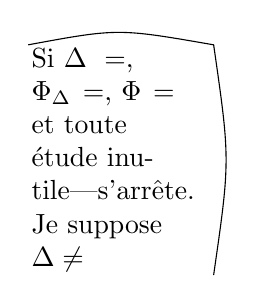
\begin{tikzpicture}
\node[inner sep=1pt,text width=2.2cm] (note) {Si $\Delta=\varnothing$, $\Phi_{\Delta}=\varnothing$, $\Phi=\varnothing$ et \unsure{toute} \unsure{étude} \unsure{inutile|s'arrête}. Je suppose $\Delta\ne\varnothing$};
\draw[thin] (note.north west) .. controls ([yshift=6pt]note.north) .. ([xshift=2pt]note.north east) .. controls ([xshift=8pt]note.east) .. ([xshift=2pt]note.south east);
\end{tikzpicture}}}

Considérons alors
\[
\begin{aligned}
\unsure{\Phi^{\prime *}|\Phi^{!*}}_0&=\deleted{\unsure{\Delta\setminus\Phi}}(\Phi_{\Delta})_0\setminus\Phi_0=\Delta\setminus\Phi_0\\
\Phi^{\prime *}_1&=(\Phi_{\Delta})_1\setminus\Phi_1
\end{aligned}
\]

Soit de plus, \deleted{si $\Delta\ne\varnothing$ (i.e. $\Phi\ne\varnothing$)}
\[
a=\mathrm{or}(\Delta),\quad b=\mathrm{ex}(\Delta)
\]
et soit
\[
\begin{aligned}
\unsure{\mathcal{M}|M}_{<a}&=\{X\in M\mid X<a\}\\
\mathcal{M}_{>b}&=\{X\in M\mid X>b\}
\end{aligned}
\]
Par Hyp., $\mathcal{M}_{<a}$ est $\varnothing$ sss $a$ est un plus petit élément de $\unsure{L|\mathcal{L}}$, et $\mathcal{M}_{>b}$ est vide \unsure{ssi|sss} $b$ est un plus grand élément de $L$. Ceci dit, on trouve \unsure{aussitôt}
\[
\mathrm{Cosupp}^{\circ}(\Phi)=\mathrm{Omb}^{\circ}(\Phi^{\prime *}_{\deleted{\unsure{1}}})\cup\mathcal{M}_{<a}\cup\mathcal{M}_{>b}
\]
(réunions disjointes), tandis que
\[
\mathrm{Omb}^{\circ}(\Phi^{\prime *})\overset{\mathrm{def}}{=}\bigcup_{X\in\Phi^{\prime *}}\mathrm{Omb}^{\circ}(X)
\]
\margin{\uline{réunion}\newline\uline{disjointe}}
